%% This is an example first chapter.  You should put chapter/appendix that you
%% write into a separate file, and add a line \include{yourfilename} to
%% main.tex, where `yourfilename.tex' is the name of the chapter/appendix file.
%% You can process specific files by typing their names in at the 
%% \files=
%% prompt when you run the file main.tex through LaTeX.

\singlespacing{


\chapter{Simulation Engine}

\section{Material Types}

We chose a relatively small basis set of material types which cover a range of desirable material properties for actuation and control.  The list of materials and a qualitative comparison of their properties is given in Table \ref{tab:materialTypes}.

\renewcommand{\arraystretch}{1.5}
%http://tex.stackexchange.com/questions/98388/how-to-make-table-with-rotated-table-headers-in-latex
\begin{table}[h] \label{tab:materialTypes}
    \centering
    \caption{Basis Set of Material Types.}
\begin{tabular}{ll | m{4cm} | *{7}{c} }
    \\
    \multicolumn{2}{c}{Function}  & \multicolumn{1}{c}{Example Materials}
        & \mcrot{1}{l}{60}{Cost} & \mcrot{1}{l}{60}{Strength} & \mcrot{1}{l}{60}{Stiffness} & \mcrot{1}{l}{60}{Fracture Resistance} & \mcrot{1}{l}{60}{Heat Resistance} & \mcrot{1}{l}{60}{Density} & \mcrot{1}{l}{60}{Magnetic Coercivity}\\
    \midrule \midrule

    \multirow{4}{*}{\rotatebox{90}{\textbf{\small{\hspace{17pt}Structural}}}}
    & Insulating & Plastics&
        x & x & x & xxx & x & xxx & -\\
    & Non-Insulating &   Metals  &
        xx & xxx & xxx & xx & xxx 
        & xx & -\\
    & Heat-Resistant&     Inconel, Alumina&
        xxxx &xx &xxxx &x &xxxx &xx & -\\
    \midrule
    \multirow{4}{*}{\rotatebox{90}{\textbf{\small{\hspace{18pt}Flexible}}}}
    & Insulating & Rubber
        & x & x & - & - & x 
        & - & x \\
    & Conductive & Metal wire   
        & x & x & - & - & x 
        & - & x\\
    & Hinge&    Metal flexure   
        & - & - & x & - & - 
        & - & -\\
        
      \midrule
     \multirow{4}{*}{\rotatebox{90}{\textbf{\small{\hspace{14pt}Conductive}}}}
    & General Purpose & Copper
        & x & x & - & - & x 
        & - & x\\
    & Lightweight &    Aluminum    
        & - & - & x & - & - 
        & - & -\\
    & Resistive&    Carbon-filled ceramic
        & - & - & x & - & - 
        & - & -\\
        
        
        \midrule
     \multirow{4}{*}{\rotatebox{90}{\textbf{\small{\hspace{16pt}Magnetic}}}}
    & Hard & NdFeB (neodymium)
        & x & x & - & - & x 
        & - & x\\
    & Soft &    AlNiCo   
        & - & - & x & - & - 
        & - & -\\
    & Ferromagnetic &    Iron     
        & - & - & x & - & - 
        & - & - \\
        
          \midrule
     \multirow{4}{*}{\rotatebox{90}{\textbf{\small{\hspace{50pt}Actuators}}}}
    & Piezoelectric & PZT (lead zirconate titanate)
        & x & x & - & - & x 
        & - & x\\
    & Heat Actuator &    Parrafin Wax
        & - & - & x & - & - 
        & - & -\\
        
         \midrule
     \multirow{4}{*}{\rotatebox{90}{\textbf{\small{Logic}}}}
    & NMOS & Silicon MOSFET
        & x & x & - & - & x 
        & - & x\\
    & PMOS &    Silicon MOSFET
        & - & - & x & - & - 
        & - & -\\
    & Diode &    Silicon     
        & - & - & x & - & - 
        & - & - \\
    & Zener Diode &    Silicon     
        & - & - & x & - & - 
        & - & - \\
        
        
        
    \bottomrule
\end{tabular}
\end{table}


\section{Hello World}

Before diving into more complex models, I wrote a "hello world" simulation engine to better understand how all the pieces of simulation (electronic, mechanical, and magnetic) would come together.

\subsection{Simple Mechanical Simulation}

I started with a simple dynamic mechanical model where the forces acting on each cell in the lattice are computed based on local interactions with its six neighbors and gravity.  In the model, virtual springs and dampers constrain translational and rotational motion of a cell relative to its neighbors (Fig \ref{fig: helloWorldLocalInteraction}).  At each time step all forces acting on each cell in the lattice are summed and the position, orientation, and translational and rotational velocities of the cell are solved by Euler integration.  All cells are updated synchronously, so the order of evaluation of the cells is not important.  All physical constants used in these calculations (mass of the cell, moment of inertia, spring stiffness, damping coefficient) are derived from the geometry and material properties of each cell.\\

In this scheme, the total force applied to the center of mass of a cell is given by:

\[ F_{total} =  \vec{f}_g+ \sum_{neighbors} \vec{f}_{neighbor}\]

With the total torque applied to the cell is given by the sum of the torques applied by its neighbors:

\[ T_{total} =  \sum_{neighbors} \tau_{neighbor} \]


\begin{figure}
  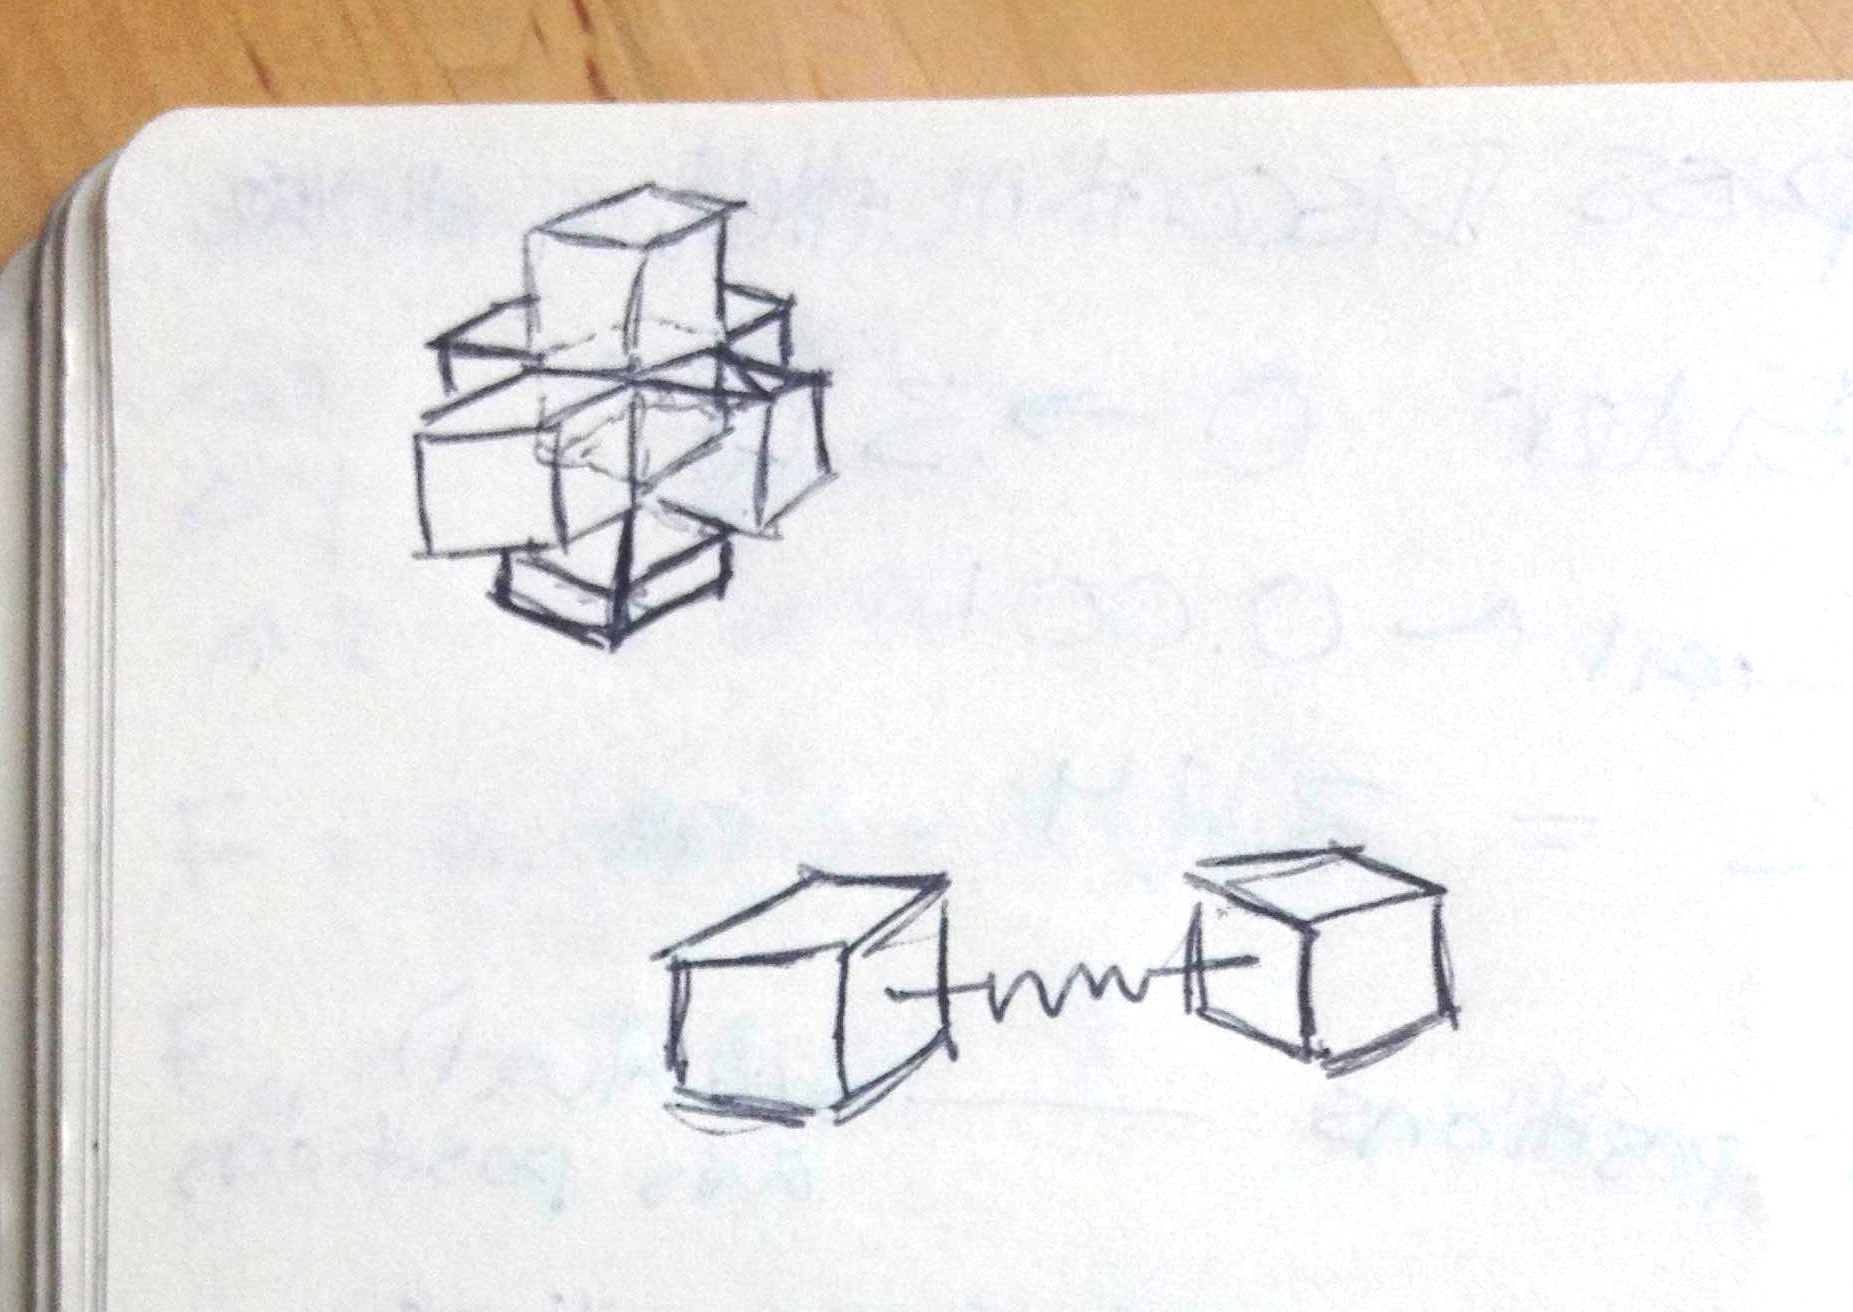
\includegraphics[width=\linewidth]{helloWorldLocalInteraction.png}
  \caption{REPLACE THIS Each cell is face-connected to its six local neighbors \textbf{(A)}.  Interaction between neighbors is modeled with springs and dampers constraining translational and rotational motion \textbf{(B)}.}
  \label{fig: helloWorldLocalInteraction}
\end{figure}

%To understand how the translational spring forces were calculated between two adjacent cells, consider the 2D case illustrated in Fig \ref{fig: helloWorldSpringSetup}.  The cells are attached by a spring with nominal length $\ell$.  Under displacement $\Delta x$ and $\Delta y$, the distance vector from cell A to cell B is given by $\vec{D}$.  Then $\Delta \ell$, the displacement of the spring from its nominal length, is given by:\\
%
%\[ \Delta \ell = \| D\| - \ell\]
%
%The force, $\vec{f}_{AB}$, exerted on cell A by a spring with stiffness $k$ is oriented in the same direction as $\vec{D}$:
%
%\[ \vec{f}_{AB} =  k (\hat{D} \Delta \ell) = k\hat{D} (\|D\| - \ell)\]
%
%An equal and opposite force, $\vec{f}_{BA}$, is applied to cell B by the spring:
%
%\[ \vec{f}_{BA} = -k\hat{D} (\|D\| - \ell)\]
%
%\begin{figure}
%  \includegraphics[width=\linewidth]{helloWorldSpringSetup.png}
%  \caption{REPLACE THIS Cubes A and B connected by spring with nominal length $\ell$ \textbf{(A)}.  The cells are displaced by $\Delta x$ and $\Delta y$ \textbf{(B)}. Spring displacement $\Delta \ell$ along $\vec{D}$ \textbf{( C )}.  $\vec{f}_{AB}$ and $\vec{f}_{BA}$ are the resulting translational spring forces applied to cells A and B, respectively \textbf{(D)}.  Larger translational displacements between neighboring cells increase the amplitude of spring forces \textbf{(E)}.}
%  \label{fig: helloWorldSpringSetup}
%\end{figure}

To understand how the translational forces were calculated between two adjacent cells, consider the 2D case illustrated in Fig \ref{fig: helloWorldSpringSetup}.  The cells are attached to each other with nominal displacement $\vec{\ell}$ from the center of cell A to the center of cell B.  If we model a two dimensional spring damper system connecting the cells, then the force applied to cell A by cell B under additional displacement $\Delta x$ and $\Delta y$ is given by:

\[ \vec{f}_{AB} =   k\left[ \begin{array}{ccc}
\Delta x \\
\Delta y \end{array} \right] - d 
\left[ \begin{array}{ccc}
v_x\\
v_y\end{array} \right] 
 \]

where k is a spring stiffness, d is a damping coefficient, and $v$ is the velocity of cell A relative to cell B.  This equation is trivially extended to the three dimensional case:\\

\[ \vec{f}_{AB} =   k\left[ \begin{array}{ccc}
\Delta x \\
\Delta y\\
\Delta z \end{array} \right] - d 
\left[ \begin{array}{ccc}
v_x\\
v_y\\
v_z\end{array} \right] 
 \]

\begin{figure}
  \includegraphics[width=\linewidth]{helloWorldSpringSetup.png}
  \caption{REPLACE THIS Adjacent cells A and B connected with nominal displacement $\vec{\ell}$ \textbf{(A)}.  The cells are additionally displaced by $\Delta x$ and $\Delta y$ \textbf{(B)}. $\vec{f}_{AB}$ and $\vec{f}_{BA}$ are the resulting translational spring-damper forces applied to cells A and B, respectively \textbf{( C )}.}
  \label{fig: helloWorldSpringSetup}
\end{figure}


The stiffness $k$ and damping coefficient $d$ of the springs and dampers are determined from the material properties of the two cells.  In the case that the two cells have different stiffnesses, a composite stiffness is calculated according to:

\[ k = \frac{2k_Ak_B}{k_A + k_B} \]

which is equivalent to two springs of half length in series.  Similarly, a composite damping coefficient is calculated by:\\

\[ d = \frac{2d_Ad_B}{d_A + d_B} \]

In addition to $\vec{f}_{AB}$, an equal and opposite force, $\vec{f}_{BA}$, is applied to cell B by the spring damper system (Fig \ref{fig: helloWorldSpringSetup} C):

\[ \vec{f}_{BA} =  -\vec{f}_{AB}\]

In addition to translational forces, neighboring cells apply torques to each other.  These torques result in rotational motion of a cell about its center of mass.  More on that soon.

%\begin{figure}
%  \includegraphics[width=\linewidth]{helloWorldSpringSetup.png}
%  \caption{REPLACE THIS Cubes A and B connected by spring with nominal displacement $\ell$ \textbf{(A)}.  The cells are further displaced by $\Delta x$ and $\Delta y$ \textbf{(B)}. Spring displacement $\Delta \ell$ along $\vec{D}$ \textbf{�}.  $\vec{f_{AB}}$ is the translational spring resulting force applied to cell A by the spring attached to cell B, force of gravity, $f_g$, also indicated \textbf{(D)}.}
%  \label{fig: helloWorldSpringRotSetup}
%\end{figure}









}
